\documentclass[fleqn,10pt]{olplainarticle}
% Use option lineno for line numbers 

\begin{document}

\begin{center}
    \Large
    \textbf{Git Assignment}  
        
    \vspace{0.4cm}
    \textbf{Kora Gwartney}

    \vspace{0.4cm}
    \textbf{CD 6000, Dr. Boult}
    
     \vspace{0.4cm}
    \textbf{09/21/2022}
\end{center}

\begin{figure}[ht]
\centering
\includegraphics[angle=90,width=0.5\linewidth]{Portrait.jpg}
\label{fig:view}
\end{figure}
\bigskip

\section*{Goals for CS 6000 }
I am working through my first year as a provisional Ph.D. student in the Security program, so I have taken the classes required to complete my provisional status. I am taking the last of the four required courses this semester and will be moved into a full Ph.D. Student status. However, Dr. Xu already has me doing a couple of introductory research projects as I am new to the interworkings of researchers outside of compliance. I seek to gain valuable insight into the generalizations on how to properly research so that as I become a researcher, I can build a research style of my own. I do not have a foundation in research, so I want to build a solid foundation to grow. Having worked in the technology field for the past ten years, I have found two rules always to be true, "you don't know what you don't know," and those who do not seek knowledge will not gain understanding. I want to be a cybersecurity expert, which means I have a lot of knowledge that I don't know, and a lot that I do know; however, I will never be stagnant in my pursuit of knowledge. This is why research is very appealing to me because now I am seeking an ability that no one might know or building upon known knowledge but has evolved.  


\subsection{Git Hub Code}

\url{https://github.com/harrisasadb/Clustering-Cyber-Security-Metrics-of-Companies}

\begin{figure}[ht]
\centering
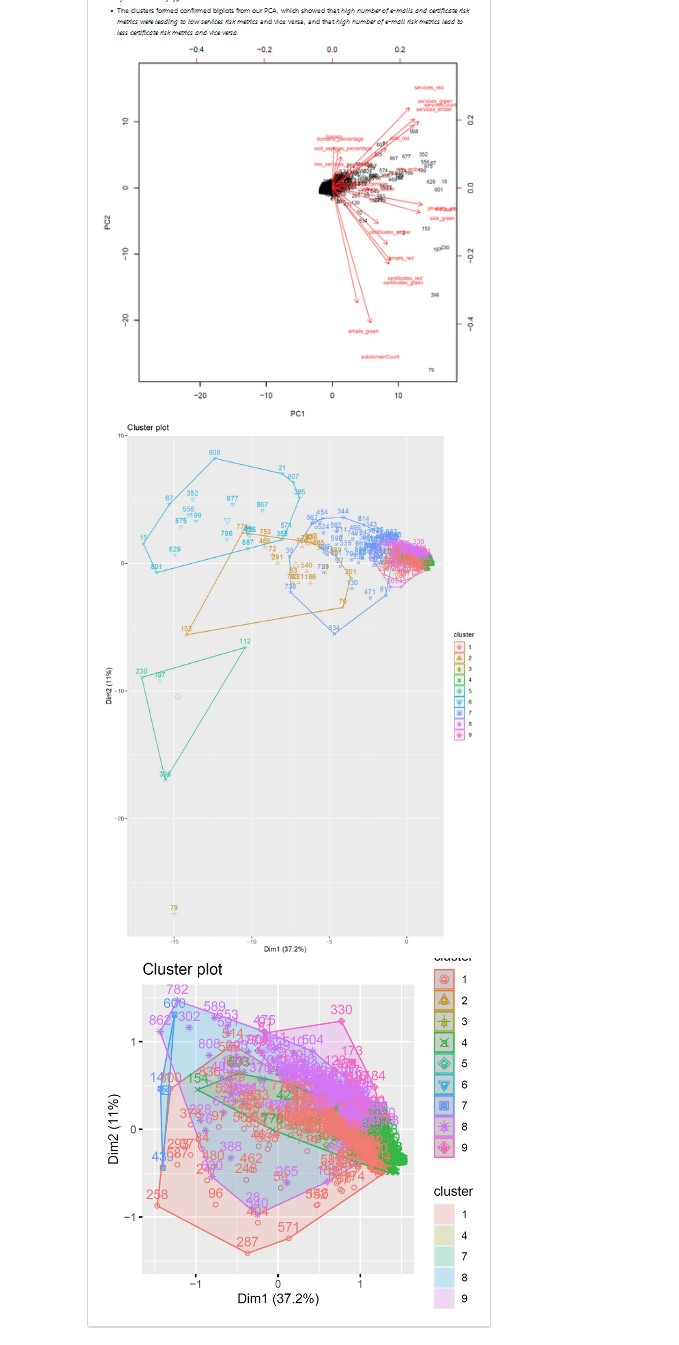
\includegraphics[angle=0,width=.7\linewidth]{GitAssignmentClustering.jpg}
\caption{Examples of Clustering Based on R code} 
\label{fig:view}
\end{figure}
\bigskip


\begin{figure}[ht]
\centering
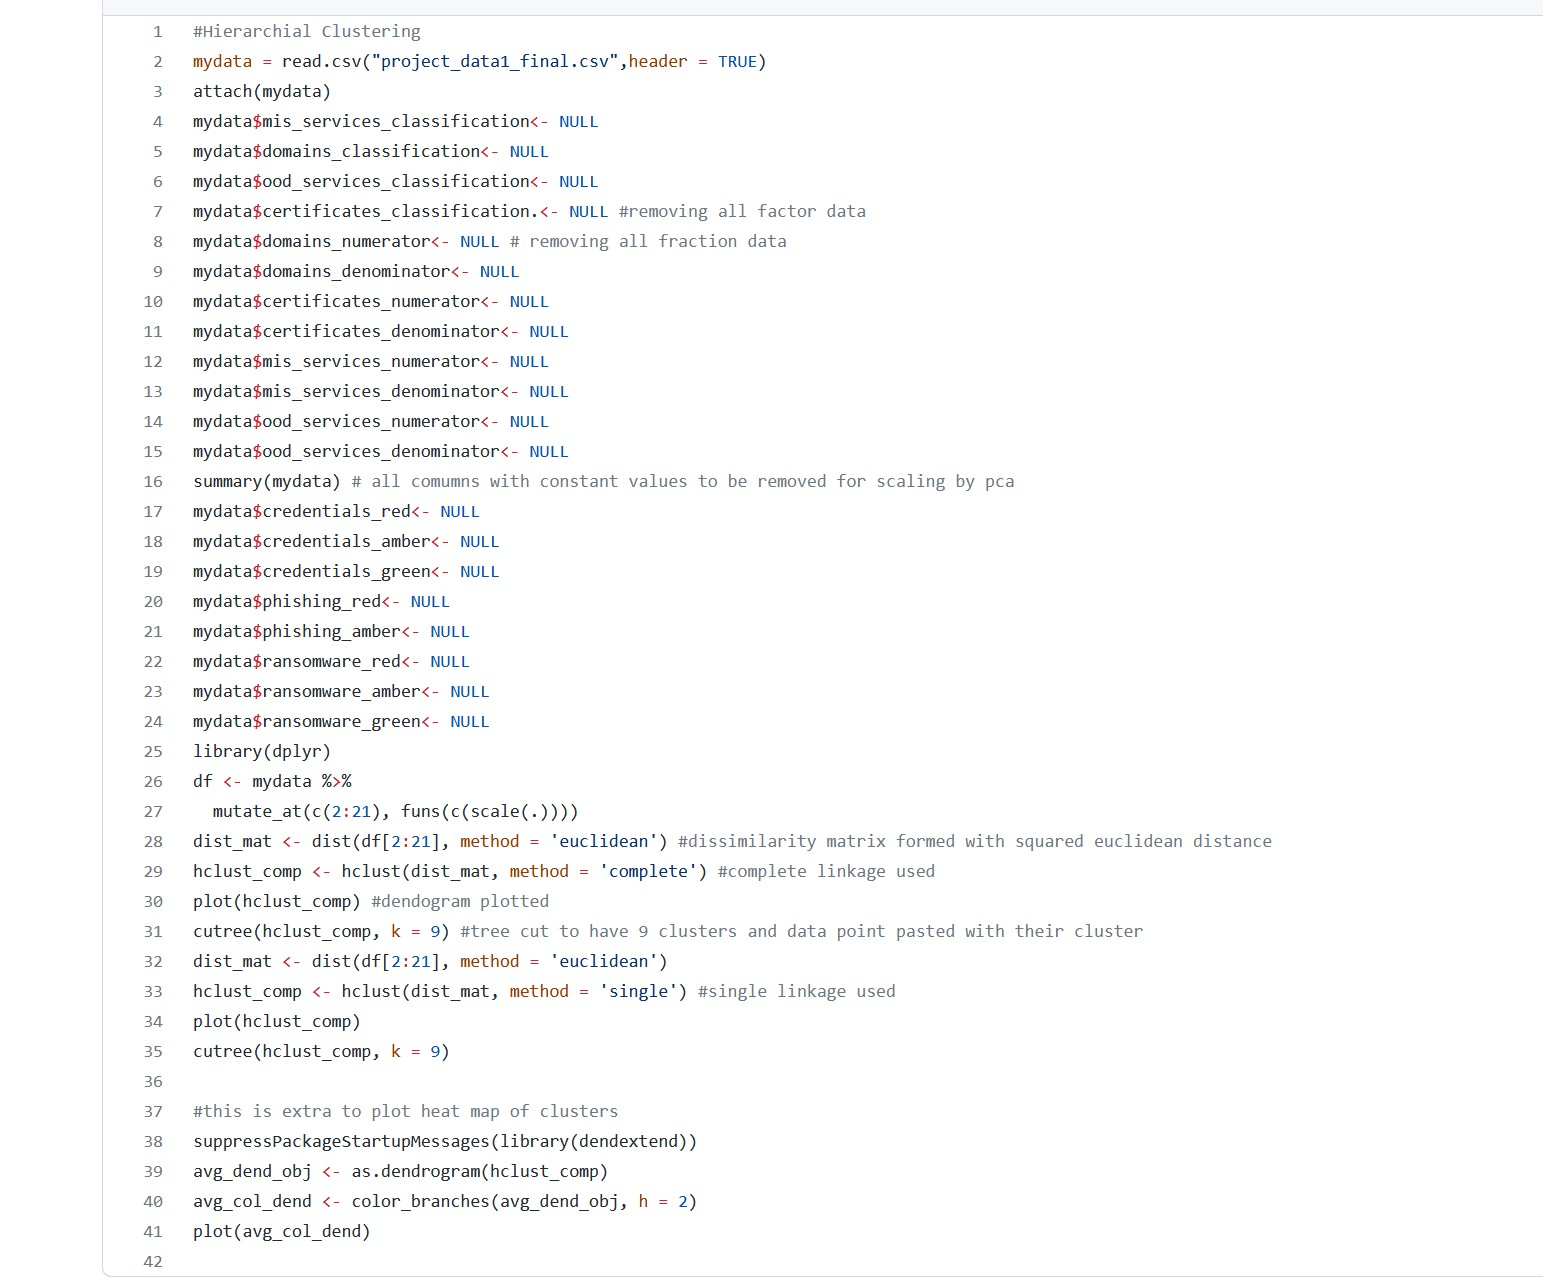
\includegraphics[angle=0,width=.7\linewidth]{R-Code-Her.jpg}
\caption{Hierarchical Clustering.R} 
\label{fig:view}
\end{figure}
\bigskip



\end{document}